\documentclass[12pt, letterpaper]{book}
\usepackage[T1]{fontenc}
\usepackage[italian]{babel}
\usepackage{hyphenat}
\hyphenation{mate-mati-ca recu-perare}
\usepackage{hyperref}
\usepackage{graphicx}

\title{Documentazione}
\author{Benedetta Vitale - Emilio Meroni}
\date{\today}

\graphicspath{{../../Immagini}}

\begin{document}

\maketitle

\tableofcontents    

\chapter{Project Plane}

\section{Introduzione}

    Questo progetto verrà svolto da Benedetta Vitale ed Emilio Meroni, entrambi studenti al terzo anno d'ingegneria informatica presso l'università di Bergamo.\\

    Il software che andremo a sviluppare è pensato per dare supporto 
    all'attività di ristorazione. In particolare, dovrà assistere alle mansioni dei camerieri, come ad esempio: prendere le ordinazioni, redigere il conto, trovare i tavoli disponibili, ecc.\\

    Abbiamo scelto questa tipologia di sistema dato che Emilio lavora, nei week-end, presso un ristorante, e gli ha incuriosito la gestione interna tramite l'utilizzo dei palmari da parte dei camerieri. 
    \begin{tabbing}
    
    \end{tabbing}
    
\section{Modello di Processo}

    Il modello di processo che seguiremo è quello della prototipazione, in particolare la prototipazione evolutiva [Figura: \ref{fig: modello_processo_evolutivo}]. Questo processo è molto utile per quanto riguarda la costruzione dell'interfaccia grafica, dato che ci aiuterà a costruire più velocemente la GUI finale, tramite diversi prototipi d'interfacce utente. La parte principale della nostra applicazione, infatti, sarà la grafica.

\begin{figure}[h]
    \centering
    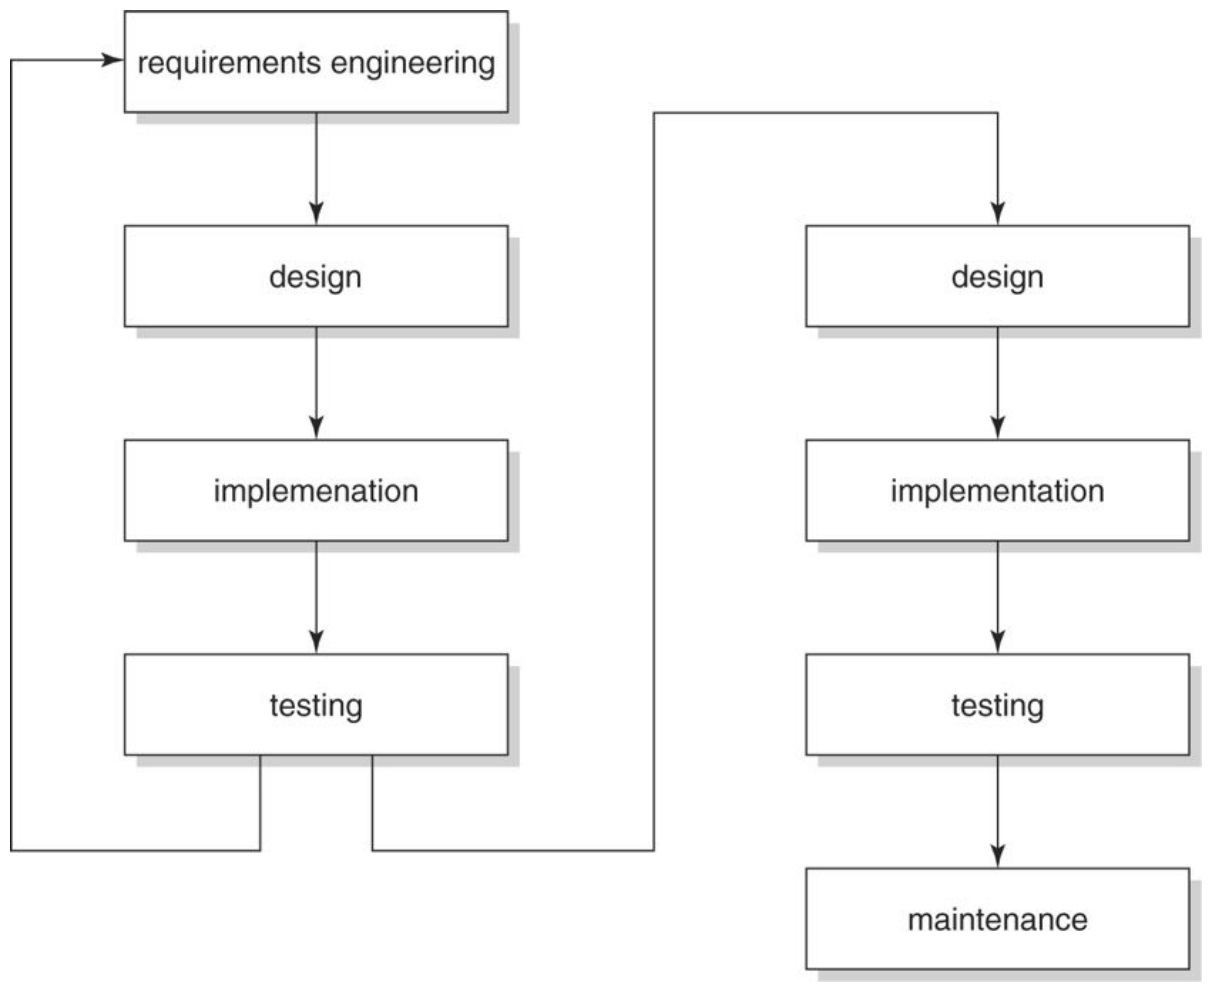
\includegraphics[width = 0.7\linewidth]{../../Immagini/Modello_Processo_Evolutivo.jpg}
    \caption{Modello Di Processo Evolutivo}
    \label{fig: modello_processo_evolutivo}
\end{figure}

\section{Organizzazione del Progetto}\label{sez: organizzazioneProgetto}

Utilizzeremo una organizzazione a tre livelli:

\begin{enumerate}
    \item Data Base
    \item Logico
    \item Presentazione
\end{enumerate}
Il livello \textit{Data Base}, come da nome, si occuperà della parte del DB, il quale sarà embedded.

Il livello \textit{Logico}, possiamo posizionarlo graficamente tra il livello Data Base e quello Presentazione. Funge da intermediario tra i due livelli e fornisce gli oggetti principali per la gestione dell'applicazione.

L'ultimo livello, quello di \textit{Presentazione}, sarà quello visto dall'utente che usufruirà dell'applicazione. Possiamo definirlo come il livello più esterno dove i dati verranno presentati in modo grafico e, la gestione dei tavoli e delle comande sarà fatta in modo interattivo.\\

Il progetto verrà suddiviso in:
\begin{itemize}
    \item \textbf{Documentazione}; questa parte verrà svolta da entrambe le figure coinvolte nel progetto. 
    \item \textbf{Progettazione desing}; parte eseguita da Benedetta, che apprezza particolarmente questo ambito.
    \item \textbf{Codifica desing}; questa porzione verrà eseguita principalmente da Emilio, dato che ha una maggiore esperienza sulla programmazione.
    \item \textbf{Codifica parte logica} e \textbf{data base}; le quali verranno scritte sia da Benedetta e sia da Emilio.
\end{itemize}

\section{Standard, Linee guida, Procedure}

Per la parte della stesura della documentazione si è scelto di utilizzare un tool molto utile nella scrittura di documenti professionali, \textit{LaTeX}. Scelta quasi obbligata, derivata dall'utilizzo di \textit{GitHub} insieme al programma di scrittura precedente \textit{Microsoft Word}; il quale ha causato difficoltà nei "merge" su \textit{GitHub}.\\

Mentre, per la parte di \textit{codifica} abbiamo scelto di utilizzare lo standard definito da \textit{Java}\footnote{Standard di Java si possono trovare su questo \href{https://www.oracle.com/java/technologies/javase/codeconventions-contents.html}{\underline{sito}}}. In primo luogo perché l'IDE utilizzato per la parte di programmazione è \textit{Eclipse}, il quale fornisce strumenti per la formattazione e nominazione di metodi in modo automatico secondo gli standard di \textit{Java}; inoltre, non avendo entrambi molta esperienza ci è venuto comodo utilizzare uno dei pochi standard di codificha che conosciamo.\\

Lo strumento che utilizzeremo per la condivisione della documentazione e del codice sarà, come già anticipato, la piattaforma di condivisione \textit{GitHub}.

\section{Attività di Gestione}

La priorità fissata per questo progetto sarà quella di avere una documentazione dettagliata, e, specialmente, di avere un project plane completo per l'inizio del mese di dicembre. Parellamente alla stesura di quest'ultimo si è deciso di dedicare, almeno una volta a settimana, del tempo sulla parte di progettazione. 


\section{Rischi}

In questa sezione si discutono i rischi che potrebbero verificarsi durante lo sviluppo del progetto. 

Un primo rischio, evidenziato da entrambe le parti, sono le difficoltà che potrebbero verificarsi nell'utilizzo di \textit{windows builder} (plugin che consente la costruzione dell'interfaccia utente su \textit{Eclipse}), dovuta a una bassa conoscenza del tool. Un probabile "effetto" sarà quello di allungare i tempi di codifica sul modulo di presentazione.

\section{Personale}
Il numero di persone che lavoreranno a questo progetto sarà molto ristretto, nello specifico sono: 
\begin{itemize}
    \item Benedetta Vitale
    \item Emilio Meroni
\end{itemize}
I quali participeranno in modo equo a quasi tutte le attività. Si è deciso che si lavorerà spesso in coppia, in particolar modo sulla parte di programmazione della GUI, dato che la parte grafica su \textit{Java} non è mai stata approfondita da entrambe le parti, e questo progetto ha una parte di grafica molto importante.
     

\section{Metodi e Tecniche}

Per ogni nuova modifica aggiunta al progetto, prima di eseguire il "merge" su \textit{GitHub}, la verificheremo tramite dei test. Sulla parte grafica il test verrà eseguito in modo visivo, tramite l'esecuzione del programma.
Se questo funzionerà ancora si procederà con l'aggiunta di nuove modifiche, così da avere sempre un codice eseguibile.

\section{Garanzia e Qualità}

Il programma dovrà essere utilizzato in ristoranti, e in particolare, dal personale che prenderà le ordinazioni. Quindi dovrà essere di \textit{facile} utilizzo, con un focus maggiore sulla funzionalità che sull'estetica. Un'altra qualità che dovrà garantire è la \textit{prevenzione di errori} da parte degli utenti, come ad esempio il "miss-click" (click errati o accidentali).\\

In particolare abbiamo evidenziato quattro qualità che il sistema dovrà possedere:

\begin{enumerate}
    \item \textbf{Semplice}: Il programma sarà scritto per avere poche sezioni scritte e di facile comprensione, anche per chi si approccia al programma per la prima volta. Si utilizzeranno poche schermate che contengono tutto il necessario per le \textit{macro} operazioni definite.
    \item \textbf{Intuiblile}: L'utilizzo dei colori per indicare gli stati dei \textit{tavoli}, in particolare si è deciso che: per i \textit{tavoli liberi} si utilizzerà il colore verde, per i \textit{tavoli occupati} il colore rosso e per i \textit{tavoli da pulire} l'arancione [Figura: \ref{fig: es_bottoni}].
    \item \textbf{Prevenzione Errori}: Per la prevenzione degli errori si utilizzeranno schermate \textit{pop-up}, per la convalida degli input.
    \item \textbf{Veloce}: Con questo termine si indica che il programma, che verrà utilizzato da dispositivi touch, dovrà essere principalmente composto da bottoni che minimizzano i tempi di utilizzo, puntando a un uso minimo della tastiera. Comportando un'esperienza più agevole per l'utente.
\end{enumerate}

\begin{figure}[h]
    \centering
    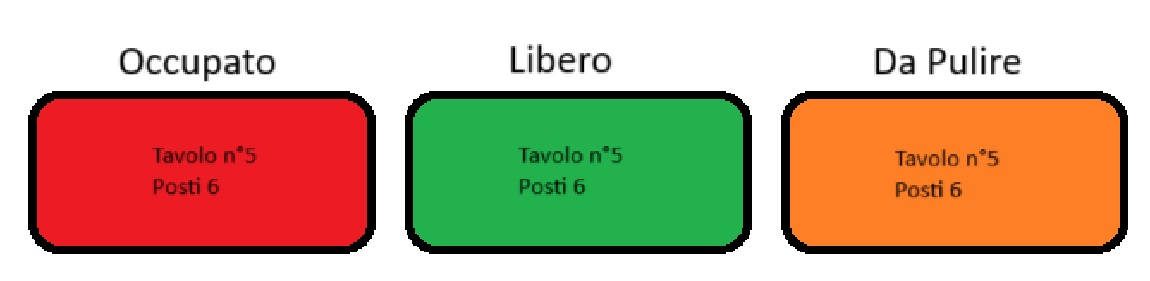
\includegraphics[width=0.6\linewidth]{Esempio_Bottoni.jpg}
    \caption{Esempio di colorazione dei bottoni per i tavoli}
    \label{fig: es_bottoni}
\end{figure}


\section{Workpackages}

I moduli presenti in questo progetto, come già anticipato parzialmente nella sezione \ref{sez: organizzazioneProgetto}, saranno:
\begin{itemize}
    \item \textbf{Documentazione}
    \item \textbf{Codifica desing}
    \item \textbf{Codifica parte logica}
    \item \textbf{Codifica data base}
\end{itemize}

L'organizzazione dei pacchetti di lavoro, presenti su \textit{GitHub}, sarà suddivisa in cartelle, per la parte di codifica raggrupperemo i diversi moduli in unico folder; mentre, la documentazione sarà posizionata in una cartella a parte.\\

Oltre ad avere queste directory, si avrà una parte dedicata ai modelli \textit{ER}(riguardanti il data base) e una per la parte \textit{UML} contenente tutti grafici per la progettazione. 

\section{Risorse}

Gli strumenti che verranno adottati in questo progetto saranno:
\begin{itemize}
    \item Per la parte di \textbf{codifica}, come già detto in precedenza, l'IDE \textit{Eclipse}, uno strumento specifico per la scrittura di codice e gestione di progetti \textit{Java}.
    \item In \textbf{scrittura} si utilizzerà l'editor di testo open source \textit{VS Code}, con l'estensione \textit{LaTeX Workshop}, per la scrittura di documenti in formato \textit{LaTeX}. Contribuendo garantire una presentazione accurata dei documenti.
    \item Infine, riguardo agli strumenti di \textbf{Software Configuration Management}, adotteremo \textit{GitHub}. Questa piattaforma sarà impiegata principalmente per la condivisione, gestione e tracciamento delle modifiche al software, oltre che per la documentazione. 

\end{itemize}

\section{Budget}

    Per quanto riguarda il bilancio, si è previsto un tempo totale di 80 ore lavorative. Con una forte attenzione sulla parte di documentazione (comprendendo anche la parte di documentazione del codice), rispetto a quella di codifica.\\

    In prima approssimazione possiamo definire una divisione del tempo come mostrato in figura [\ref{fig: diagramma_gant}]. 
    \begin{figure}[h]
        \centering
        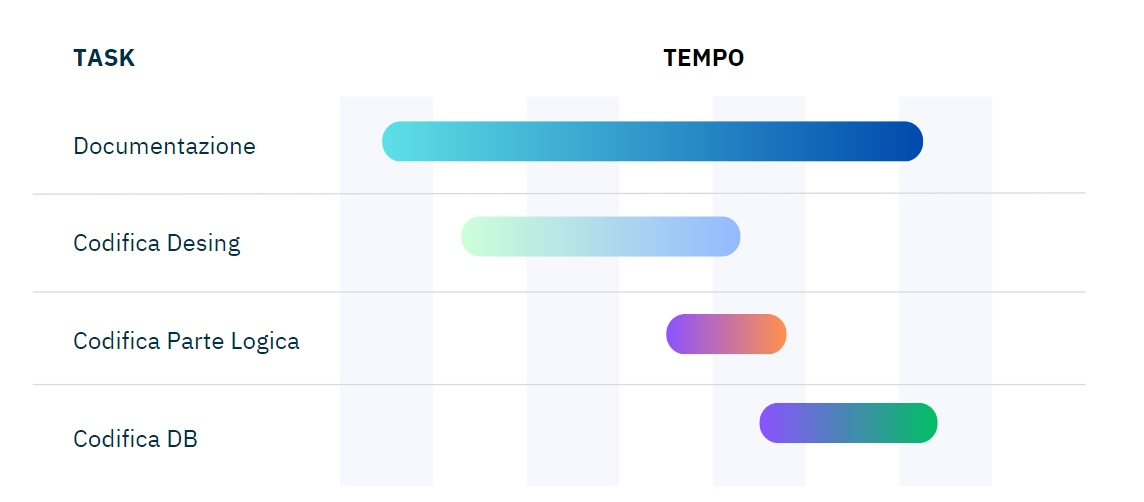
\includegraphics[width = 1\linewidth]{Diagramma_Gant.jpg}
        \caption{Diagramma di Gant}
        \label{fig: diagramma_gant}    
    \end{figure}

\section{Cambiamenti}

    Per quanto riguarda le modifiche che verranno richieste si seguirà la seguente scaletta: inizialmente si verificherà la fattibilità, in caso negativo si cercheranno altre soluzioni che vadano incontro al cliente. Mentre, se si accettano, verrà creato un "branch" sulla piattaforma di \textit{GitHub}. Da qui si aggiornerà la documentazione e i vari diagrammi \textit{UML}, in seguito si procederà alle modifiche del codice. Infine prima di eseguire il "merge" delle modifiche con il \textit{main branch}, si eseguiranno dei test di verifica della funzionalità e di correttezza.

\section{Consegna}


    In questa sezione si discutono i metodi e le scadenze di consegna del progetto, in particolare la consegna si dividerà in due fasi:


    \begin{itemize}
        \item Consegna del \textbf{Project Plane}, il quale dovrà essere consegnato circa un mese prima del primo esame scritto, che si svolgerà nel mese di gennaio; quindi, per il mese di dicembre si dovrà effettuare la prima consegna.
        \item Consegna del \textbf{Progetto}, quest'ultimo avrà una scadenza più lunga, infatti, l'ultimo giorno di consegna sarà cinque giorni prima dell'esame orale.
    \end{itemize}
    Per quanto riguarda i metodi di consegna si dovrà condividere con il professore Gargantini la repository di \textit{GitHub} contenente il progetto. Per la consegna della documentazione si dovrà indicare nel file \textit{readMe}, della repository, la posizione del project plane. Mentre, per la consegna del progetto si dovrà creare un \textit{issue}, intitolata “Approvazione Progetto” e assegnarla al professore.

% \chapter{Specifiche dei Requisiti}

% \begin{figure}[ht]
%     \centering
%     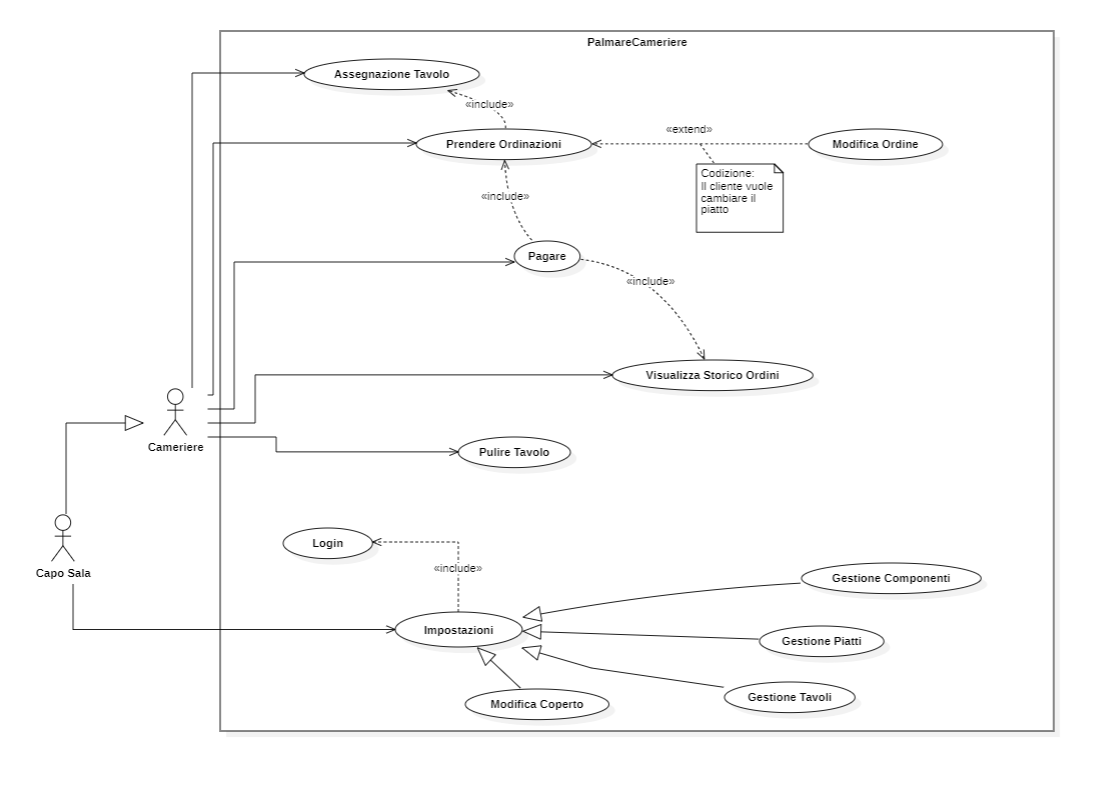
\includegraphics[width=1\linewidth]{../../UML/Diagrammi/Use_Case_Diagram.png}
%     \caption{Use Case Diagram}
%     \label{fig: use_case_diagram}
% \end{figure}

\end{document}